\documentclass[twoside,11pt]{article}

\usepackage{blindtext}

% Any additional packages needed should be included after jmlr2e.
% Note that jmlr2e.sty includes epsfig, amssymb, natbib and graphicx,
% and defines many common macros, such as 'proof' and 'example'.
%
% It also sets the bibliographystyle to plainnat; for more information on
% natbib citation styles, see the natbib documentation, a copy of which
% is archived at http://www.jmlr.org/format/natbib.pdf

% Available options for package jmlr2e are:
%
%   - abbrvbib : use abbrvnat for the bibliography style
%   - nohyperref : do not load the hyperref package
%   - preprint : remove JMLR specific information from the template,
%         useful for example for posting to preprint servers.
%
% Example of using the package with custom options:
%
% \usepackage[abbrvbib, preprint]{jmlr2e}


%\usepackage{todonotes}
\usepackage{graphicx}
\usepackage{subcaption}
\usepackage{jmlr2e}
% Heading arguments are {volume}{year}{pages}{date submitted}{date published}{paper id}{author-full-names}
\usepackage{lastpage}
\jmlrheading{26}{2025}{1-\pageref{LastPage}}{8/24; Revised
11/25}{11/25}{24-1353}{Sarah Segel, Helena Graf, Edward Bergman, Kristina Thieme, Marcel Wever, Alexander Tornede, Frank Hutter, Marius Lindauer}

% Short headings should be running head and authors last names
\ShortHeadings{\Deepcave: A Visualization and Analysis Tool for Automated Machine Learning}{Segel, Graf, Bergman, Thieme, Wever, Tornede, Hutter, and Lindauer}
\firstpageno{1}

\begin{document}

\newcommand{\HPO}{HPO\xspace}
\newcommand{\ML}{ML\xspace}
\newcommand{\AutoML}{AutoML\xspace}
\newcommand{\Deepcave}{DeepCAVE\xspace}

\title{\Deepcave: A Visualization and Analysis Tool for Automated Machine Learning}

\author{\name Sarah Segel$^1$ \email s.segel@ai.uni-hannover.de
       \AND
       \name Helena Graf$^1$ \email h.graf@ai.uni-hannover.de
       \AND
       \name Edward Bergman$^2$ \email bergmane@cs.uni-freiburg.de
       \AND
       \name Kristina Thieme$^1$ \email kristina.thieme@stud.uni-hannover.de
       \AND
       \name Marcel Wever$^{1,4}$ \email m.wever@ai.uni-hannover.de
       \AND
       \name Alexander Tornede$^1$ \email a.tornede@ai.uni-hannover.de
       \AND
       \name Frank Hutter$^{2,3}$ \email fh@cs.uni-freiburg.de
       \AND
       \name Marius Lindauer$^{1,4}$ \email m.lindauer@ai.uni-hannover.de
       \\
       \addr $^1$Leibniz University Hannover, 
       \addr $^2$University of Freiburg,
       \addr $^3$ELLIS Institute T{\"u}bingen,
       \addr $^4$L3S Research Center
       }

\editor{Zeyi Wen}

\maketitle

\begin{abstract}%   <- trailing '%' for backward compatibility of .sty file
Hyperparameter optimization (\HPO), as a central paradigm of AutoML, is crucial for leveraging the full potential of machine learning (ML) models; yet its complexity poses challenges in understanding and debugging the optimization process. 
We present \Deepcave, a tool for interactive visualization and analysis, providing insights into \HPO. 
Through an interactive dashboard, researchers, data scientists, and ML engineers can explore various aspects of the \HPO process and identify issues, untouched potentials, and new insights about the ML model being tuned. 
By empowering users with actionable insights, \Deepcave contributes to the interpretability of \HPO and ML on a design level and aims to foster the development of more robust and efficient methodologies in the future.
\end{abstract}

\begin{keywords}
  Automated machine learning, hyperparameter optimization, interpretable machine learning, human-centered machine learning, visualization
\end{keywords}

\section{Introduction}

Modern methods for hyperparameter optimization (\HPO) encompass a diverse range of approaches beyond grid and random search~\citep{turner-neuripscomp21a,bischl-dmkd23a}.
However, their lack of insight and transparency can lead to a lack of trust by users~\citep{drozdal-iui20a} and make debugging such methods and their application difficult.
We introduce \Deepcave, a visualization and analysis tool for \HPO, aiding in understanding and debugging the application of \HPO.
At present, \HPO is our main priority, wherein metadata in the format of configurations and performance values is generated in an iterative process, as many automated machine learning (\AutoML) packages do, such as Auto-Sklearn~\citep{feurer-jmlr22a}, TPOT~\citep{olson-automl19b}, AutoPyTorch~\citep{zimmer-tpami21a} or Auto-Keras~\citep{jin-sigkdd19a}.
Similarly, leveraging \Deepcave for neural architecture search (NAS)~\citep{elsken-arxiv22a} or combined algorithm selection and hyperparameter optimization~\citep{thornton-kdd13a} is possible by encoding architectural decisions, algorithmic choices, or machine learning pipelines as part of the configuration.
Advances in machine learning and \HPO, including multi-objective or multi-fidelity methods, challenge interpretation and analysis tools.
\Deepcave addresses this by offering support for multiple objectives and fidelities, with specific visualizations tailored to the different scenarios.
This tightly interacts with the vision of a more human-centered approach of AutoML~\citep{lindauer-icml24a}, in which users can learn from \HPO and ultimately even integrate their expertise into the system~\citep{hvarfner-iclr22, mallik-neurips23a}.
Moreover, to facilitate a reproducible and transparent research process, users can export visualizations to incorporate into their research papers, thereby providing insight into their \HPO process and optimized hyperparameters.

\section{Features and Usage}

\Deepcave's architecture relies upon various components, as illustrated in \autoref{fig:structure}. 
The tool is exclusively written in Python, given its prevalence as the predominant programming language in machine learning~\citep{raschka-information20}.
Built on the Dash framework~\citep{plotly-15a}, it offers users a fully interactive environment within a web browser.

\begin{figure}
    \centering
    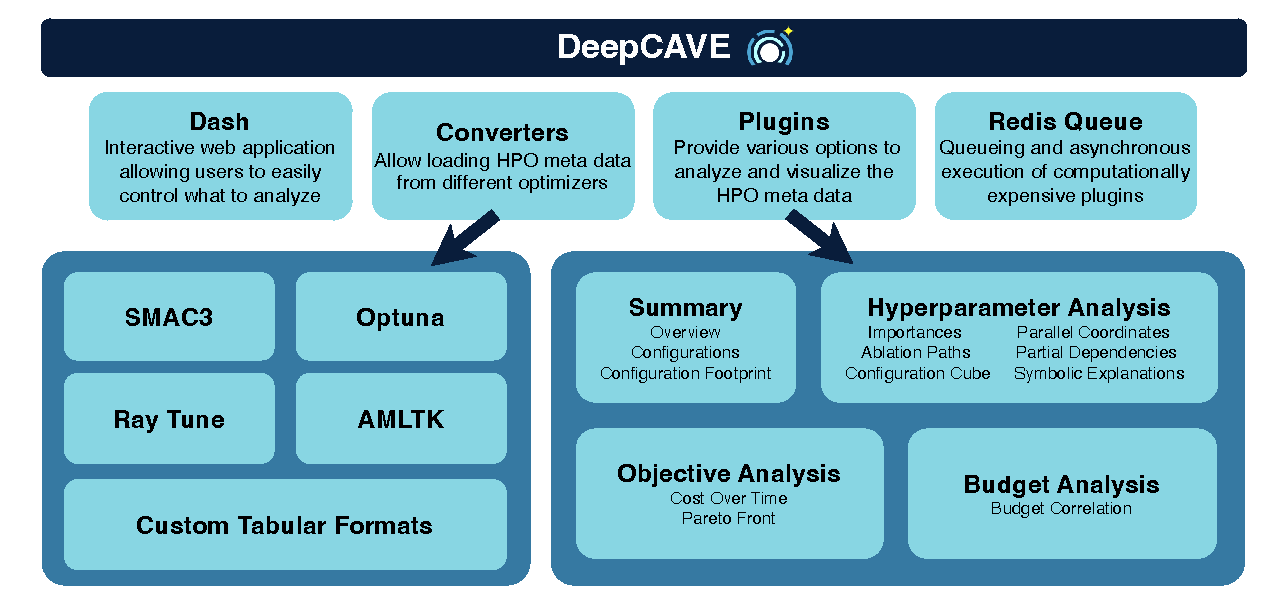
\includegraphics[width=.65\textwidth]{figures/DeepCave_Structure.drawio.pdf}
    \caption{Overview of \Deepcave's components and their functionalities.}
    \label{fig:structure}
\end{figure}

\subsection{Converters}

\Deepcave utilizes run objects as a basic unit for data interpretation, where a run can be considered an \HPO process consisting of a list of trials, each representing a hyperparameter configuration with associated objective value, budget, and seed. 
The interface allows for selection and grouping of runs, streamlining the analysis of many \HPO runs at once. 
Converters are used to access the optimizer data stored in the file system and transfer them into a run object. 
They keep track of both finished and running optimization processes that consistently write new results to disk. 
At the time of writing, \Deepcave supports loading runs created by the \HPO packages SMAC3~\citep{lindauer-jmlr22a}, Ray Tune~\citep{liaw-automl18a}, and Optuna~\citep{akiba-ickddm19a}, as well as, the \AutoML framework AMLTK~\citep{bergman2023amltk}.
Furthermore, to allow loading runs from arbitrary optimizers, \Deepcave offers a generic tabular input format, as well as a programmatic interface.

\subsection{Analysis Plugins}

\Deepcave's strength lies in its modular plugin structure, providing diverse insights into the \HPO run. 
Plugins allow analyzing overall runs, objectives, hyperparameters, and budgets through texts, tables, and Plotly~\citep{plotly-15a} visualizations. 
Dynamic filtering enables the interactive selection of certain aspects, such as specific objectives or budgets.
For computationally intensive plugins, Redis Queue~\citep{redis-queue} is leveraged for efficient queueing and asynchronous execution, ensuring a responsive user experience.

\begin{figure}
    \centering
    \begin{subfigure}[b]{0.35\textwidth}
        \centering
        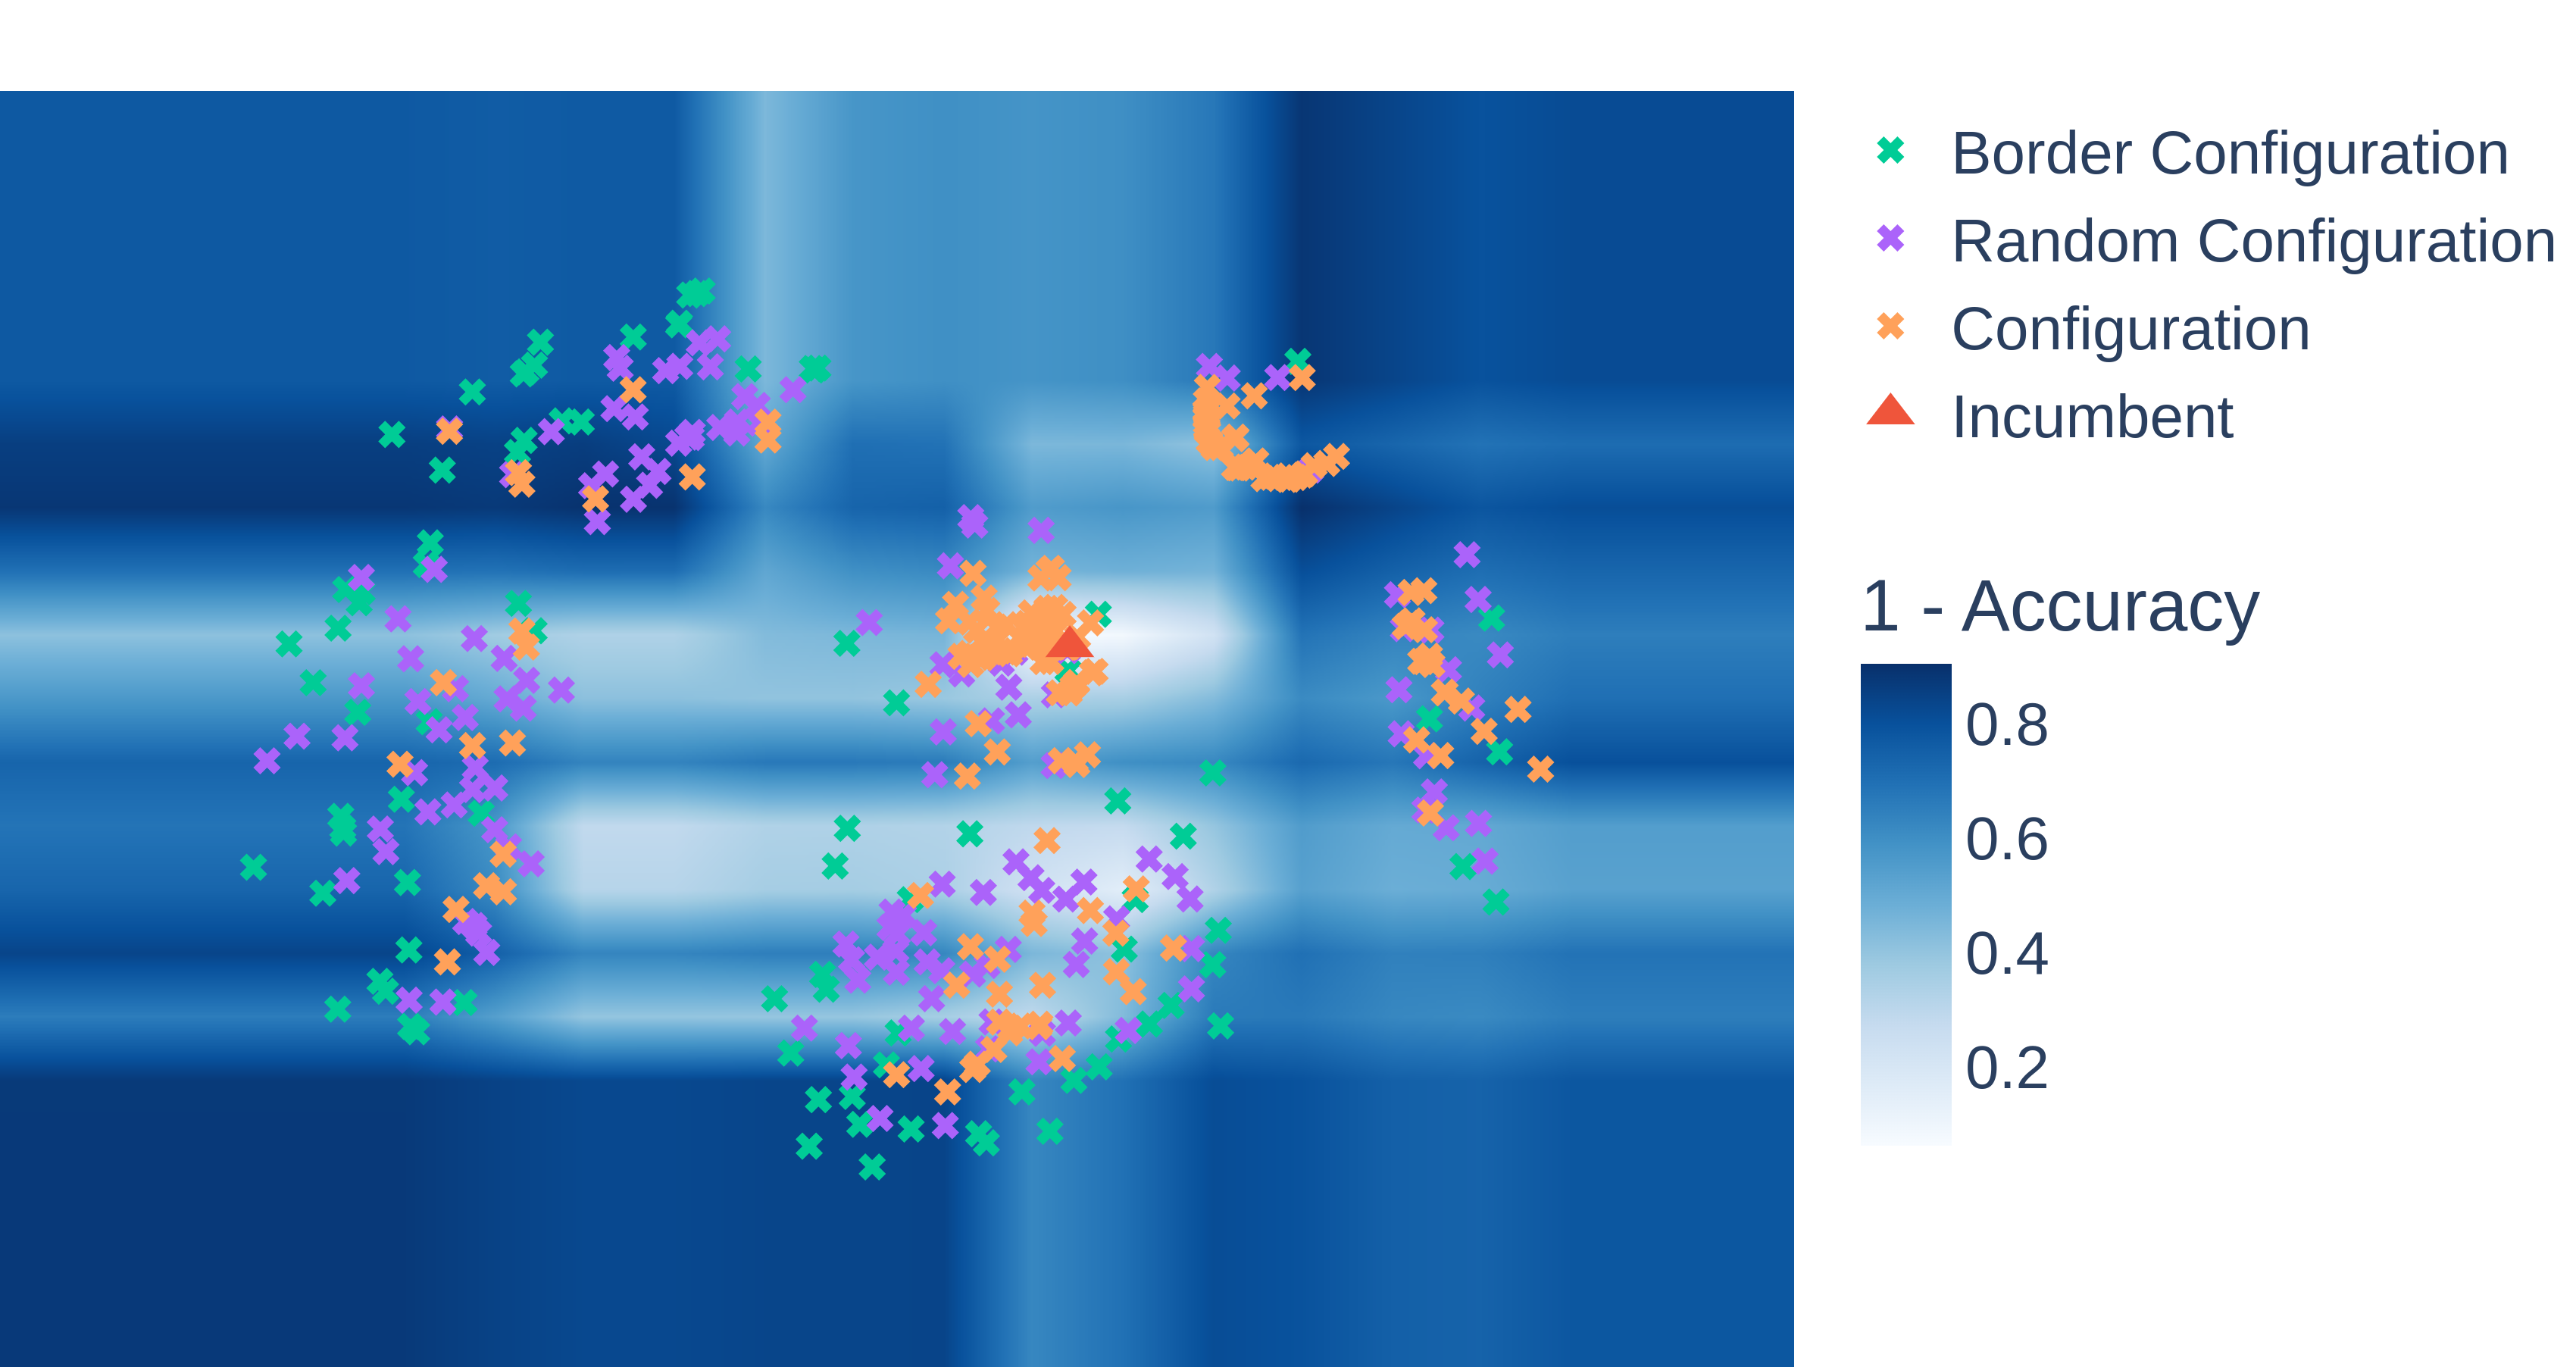
\includegraphics[width=\textwidth]{figures/Footprint.png}
        % Created with /logs/SMAC3v2/mf/ac411cecb0c431911e987eb296af869a
        \vspace{0.09\baselineskip}
        \caption{Configuration Footprint.}
        \label{fig:footprint}
    \end{subfigure}
    \begin{subfigure}[b]{0.32\textwidth}
        \centering
        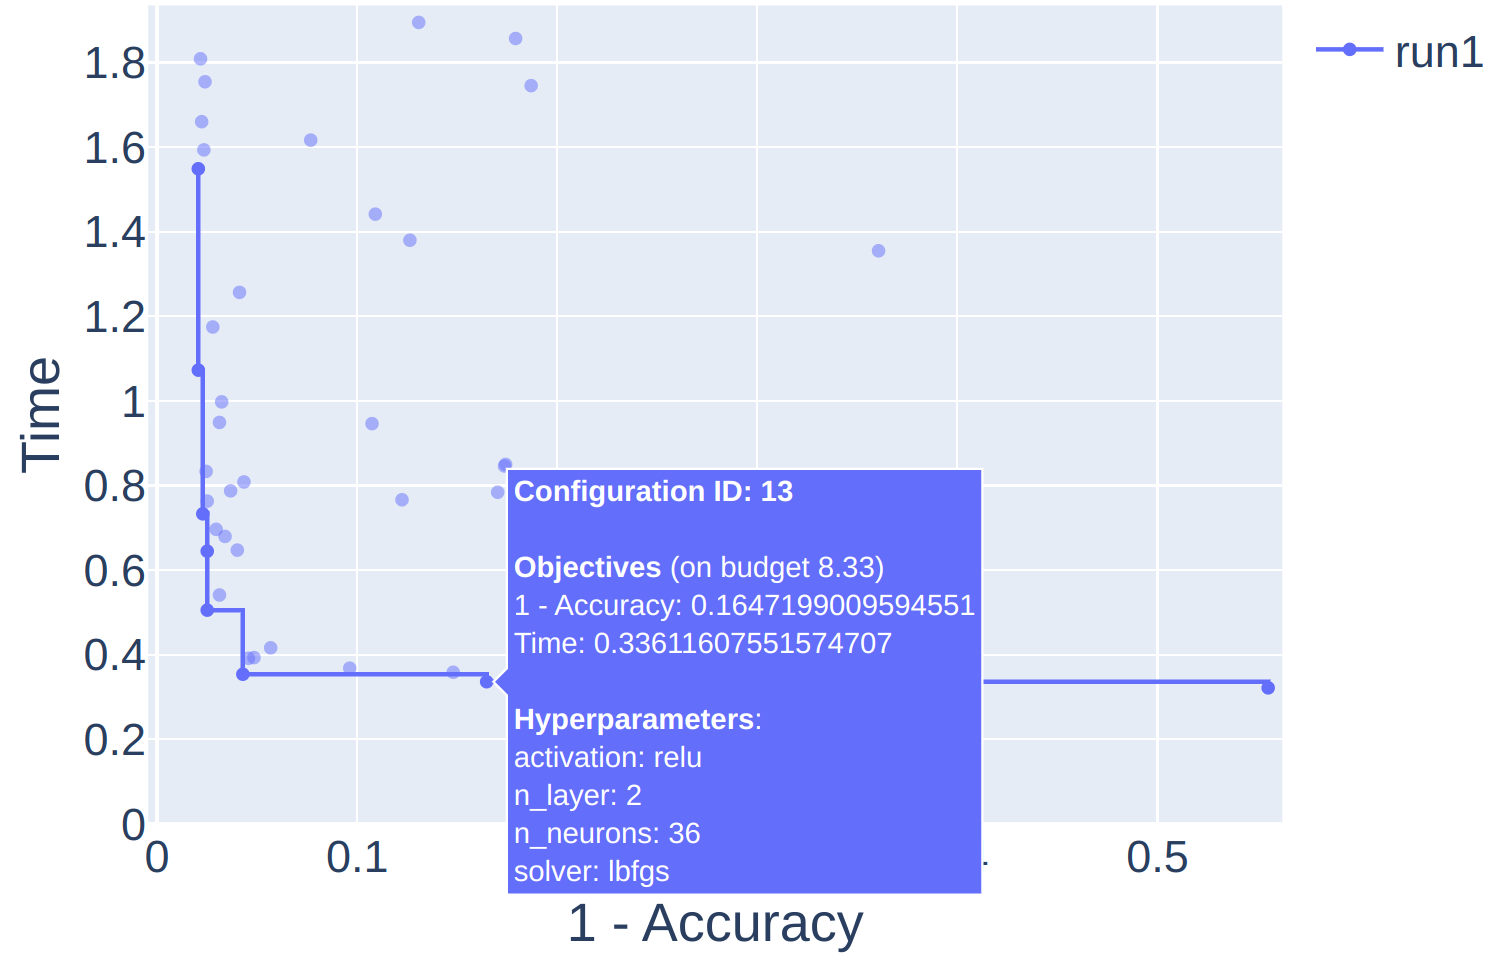
\includegraphics[width=\textwidth]{figures/Pareto.png}
        % Created with /logs/SMAC3v2/mf budget 8.33
        \vspace{-0.92\baselineskip}
        \caption{Pareto Front.}
        \label{fig:pareto-front}
    \end{subfigure}
    %\hspace{0.5\baselineskip}
    \begin{subfigure}[b]{0.31\textwidth}
        \centering
        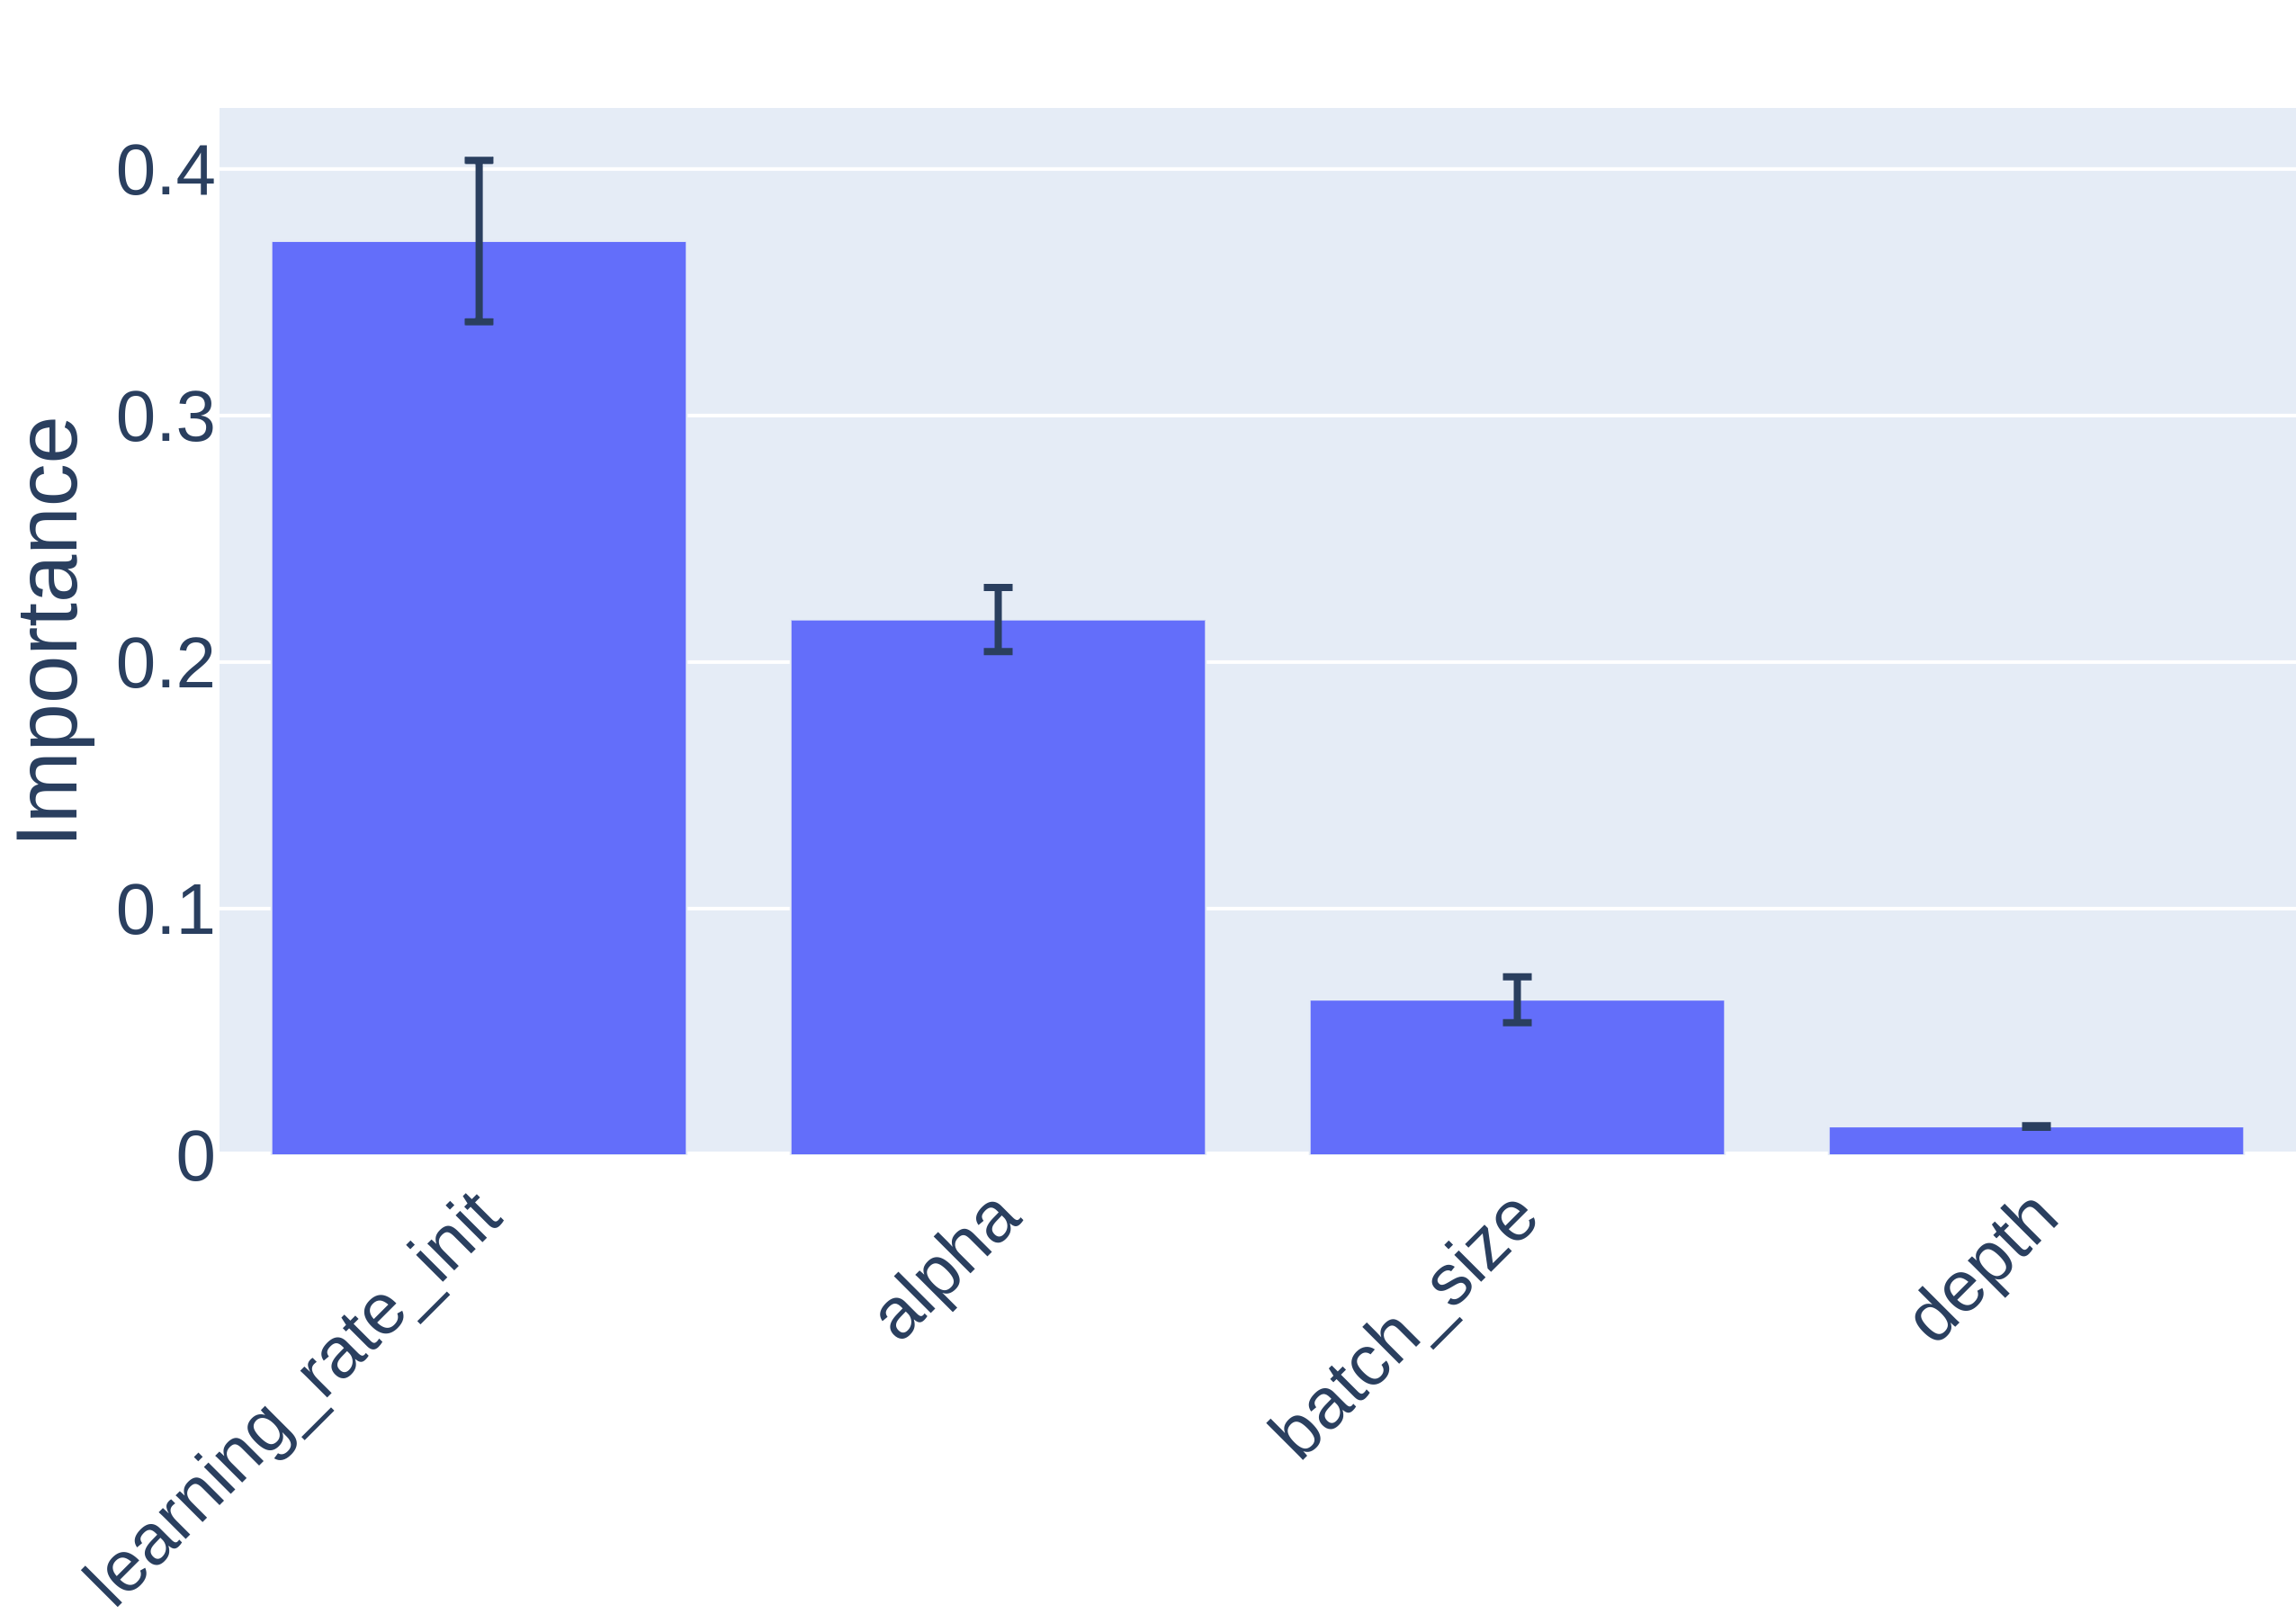
\includegraphics[width=\textwidth]{figures/Importances.png}
        % Created with /logs/SMAC3v2/mlp/run_2 fANOVA
        \vspace{-0.91\baselineskip}
        \caption{Importances.}
        \label{fig:importances}
    \end{subfigure}
    \caption{Examples of plots produced via \Deepcave's plugins. A mouseover allows obtaining additional information, and clicking on single configurations in the plot opens the Configurations plugin, providing details regarding that configuration.}
    \label{fig:whole}
\end{figure}

\textbf{Overall Optimization Analysis} The \textit{Overview plugin} offers a holistic view, showing optimizer choice, configuration space, and trial status.
Detailed analysis of individual configurations can be performed via the \textit{Configurations plugin}.
Employing multi-dimensional scaling~\citep{kruskal-psychometrika64a, kruskal-psychometrika64b} for dimensionality reduction, the \textit{Configuration Footprint plugin} visually represents the optimizer's coverage of the configuration space~\citep{biedenkapp-lion18a}, as shown in~\autoref{fig:footprint}.
This can help to identify limited exploration, suggesting the optimizer might be stuck in a local optimum.

%\textbf{Objective Analysis} Regarding objective analysis, the \textit{Cost Over Time plugin} visualizes how objective values change over time or trials, providing insights into optimizer convergence and performance comparisons among different optimizers.
\textbf{Objective Analysis} The \textit{Cost Over Time plugin} visualizes optimization convergence, either over time or the number of trials evaluated, allowing to compare different optimization strategies such as the optimizer chosen, search space design, or other meta-level decisions. %employed in \HPO tuning.
The \textit{Pareto Front plugin} visually represents configurations that achieve different tradeoffs between conflicting objectives, such as runtime versus final loss, as shown in~\autoref{fig:pareto-front}.
%For example, the Pareto front plot in supports users in choosing a configuration when both runtime and final loss need to be considered.

\textbf{Hyperparameter Analysis} As the relationship between hyperparameter configurations and objective values constitutes a crucial aspect of \HPO, \Deepcave provides a variety of plugins in this regard.
\textit{Parallel Coordinates} plots visualize hyperparameter configurations as lines, connecting their hyperparameter values and corresponding final scores~\citep{golovin-kdd17a}. 
Additionally, \textit{Partial Dependence} plots~\citep{friedman-as01a, moosbauer-neurips21a} offer insights into the average marginal effect of single hyperparameters on the objective value. 
Moreover, \textit{Symbolic Explanations}~\citep{segel-automl23a} provide explicit formulas capturing the relationship between hyperparameter and objective values.
To understand the impact of individual hyperparameters on the objective, the \textit{Importances plugin} can be used.
With fANOVA~\citep{hutter-icml14a}, see~\autoref{fig:importances}, and local (hyper)parameter importance (LPI)~\citep{biedenkapp-lion18a}, users can explore both global and local importance.
\textit{Ablation Paths}~\citep{biedenkapp-aaai17a} provide insights into the impact of sequentially adjusting individual hyperparameter values towards the incumbent configuration. In practice, \Deepcave has been used to analyze optimization runs with up to 39 hyperparameters, confirming its scalability for high-dimensional settings.

\textbf{Budget Analysis} Effective use of multiple fidelities crucially relies on a consistent rank or performance correlation to effectively allocate more resources to better configurations.
The \textit{Budget Correlation plugin} directly visualizes this correlation between fidelities, allowing users to assess the utility of their multiple fidelities.

Although \Deepcave provides diverse analysis plugins and visualizations, their customization and composition are currently limited, outlining interesting future work.

\section{Existing Tools for Explainable \AutoML}
With the rising interest in explainability and insight into optimization processes, a number of tools aiming to fill this gap have emerged. 
Among these, XAutoML~\citep{zoller-acm23a} focuses on \AutoML and interpretability. 
Similar to \Deepcave, it provides a number of different interactive visualizations.
Notably, it allows users to extend its capabilities through custom ``cards'', similar to plugins in \Deepcave, and supports a range of common (Auto)ML libraries. 
In contrast to our tool, it lacks support for (parallel) background computation and analysis of running \HPO processes.
Further, only one \HPO run is considered at a time, making comparisons between runs cumbersome. %, and no generic input format exists.
Beyond XAutoML, platforms like RapidMiner~\citep{altair}, Google Vizier~\citep{golovin-kdd17a}, and ATMseer~\citep{wang-chi18a} cater to specific facets of \AutoML processes, such as algorithm selection, experiment tracking, and pipeline analysis, albeit often with limitations in terms of interpretability at the \HPO level or support for run comparisons. 
Similarly, tools like Optuna~\citep{akiba-ickddm19a}, IOHanalyzer~\citep{wang-acm22a}, TensorBoard~\citep{abadi-15a}, WandB~\citep{biewald-wandb20a}, MLFlow~\citep{chen-deem20a}, MLJar~\citep{plonska-21a}, SigOpt~\citep{clark-19a}, IBM AutoAI~\citep{wang-iui20ab}, Pipeline Profiler~\citep{ono-ieee21a}, iraceplot~\citep{lopezibanez-github25}, and Boxer~\citep{gleicher-cgf20a} contribute valuable insights through various forms of run analysis, visualization, and reporting. 
However, many of these tools depend on specific formats, lack extensibility, or fail to support comparisons across multiple \HPO runs.
\Deepcave distinguishes itself in this field with its focus on \HPO, interpretability, and interactivity. 
Its unique proposition lies in its ability to facilitate detailed comparisons across different \HPO runs.
Moreover, its extensive format compatibility, efficient computational parallelization, and browser-based accessibility mitigate major usability challenges found in comparable tools.

\section{Conclusion}
\Deepcave is a novel tool for interactively analyzing and explaining \HPO runs. 
%\Deepcave is built in a flexible way, featuring several components. 
It allows performing comprehensive analyses of \HPO runs concerning their hyperparameters, objectives, and budgets via an interactive dashboard running in the web browser.
\Deepcave is accessible under Apache License Version 2.0\footnote{\url{https://www.apache.org/licenses}} and can be installed via the instructions in the GitHub repository \url{https://github.com/automl/DeepCAVE}.

% Acknowledgements and Disclosure of Funding should go at the end, before appendices and references

\acks{Sarah Segel acknowledges financial support by the Federal Ministry for Economic Affairs and Energy of Germany in the project CoyPu under Grant No. 01MK21007L. Helena Graf, Alexander Tornede, Marcel Wever, and Marius Lindauer gratefully acknowledge funding by the European Union (ERC, ``ixAutoML'', grant no.101041029). Frank Hutter acknowledges funding by the European Union (ERC Consolidator Grant DeepLearning 2.0, grant no.~101045765).
Edward Bergman was partially supported by TAILOR, a project funded by EU Horizon 2020
research and innovation programme under GA No 95221. Views and opinions expressed are however those of the author(s) only and do not necessarily reflect those of the European Union or the European Research Council Executive Agency. Neither the European Union nor the granting authority can be held responsible for them.

\begin{center}
    
\includegraphics[height=2cm]{LOGO_ERC-FLAG_EU.pdf}
\end{center}
}

% Manual newpage inserted to improve layout of sample file - not
% needed in general before appendices/bibliography.

% \newpage

%\vskip 0.2in
\bibliography{strings, lib, additional, proc}



\end{document}
